\chapter{Análisis inicial del problema}
\label{ch:analisis}
En este capítulo se recoge el juego del que parte el proyecto, lo que es ARCore y como puede ayudar al juego, la propuesta inicial del juego, junto con la narrativa de éste, y por útlimo las primeras ideas sobre como ampliar el juego con realidad aumentada.

\section{Juego de partida}
El juego de partida del proyecto es Cluedo, este es un juego de mesa de estrategía y misterio que consiste en resolver un asesinato.\\

El modo de funcionamiento de dicho juego consiste en que, al empezar el asesinato ya se ha cometido con un arma y en una habitación, por lo que el objetivo principal de los jugadores es descubrir quien lo hizo, con que arma y en que habitación.\\

La forma de descubrir los datos del asesinato es investigando en las diferentes habitaciones, cada jugador puede moverse a donde la tirada de dados le permita y una vez en la habitación podrán hacer una deducción sobre dicha habitación, indicando arma y personaje, de forma que el jugador de la izquierda tiene que enseñar alguna de las cartas de la deducción si las tiene, en caso de que no lo hará el siguiente personaje y así.\\

Con esta información el jugador puede ir marcando que elementos pueden ser o no parte del asesinato, y en el momento que crea saber la solución tendrá que realizar una acusación. En caso de ser esta cierta ha ganado, y en caso contrario deja de jugar.\\

En la Figura \ref{figura-cluedo-fisico} se puede observar el juego de mesa Cluedo en formato físico.

\begin{figure}[h]
  \centering
  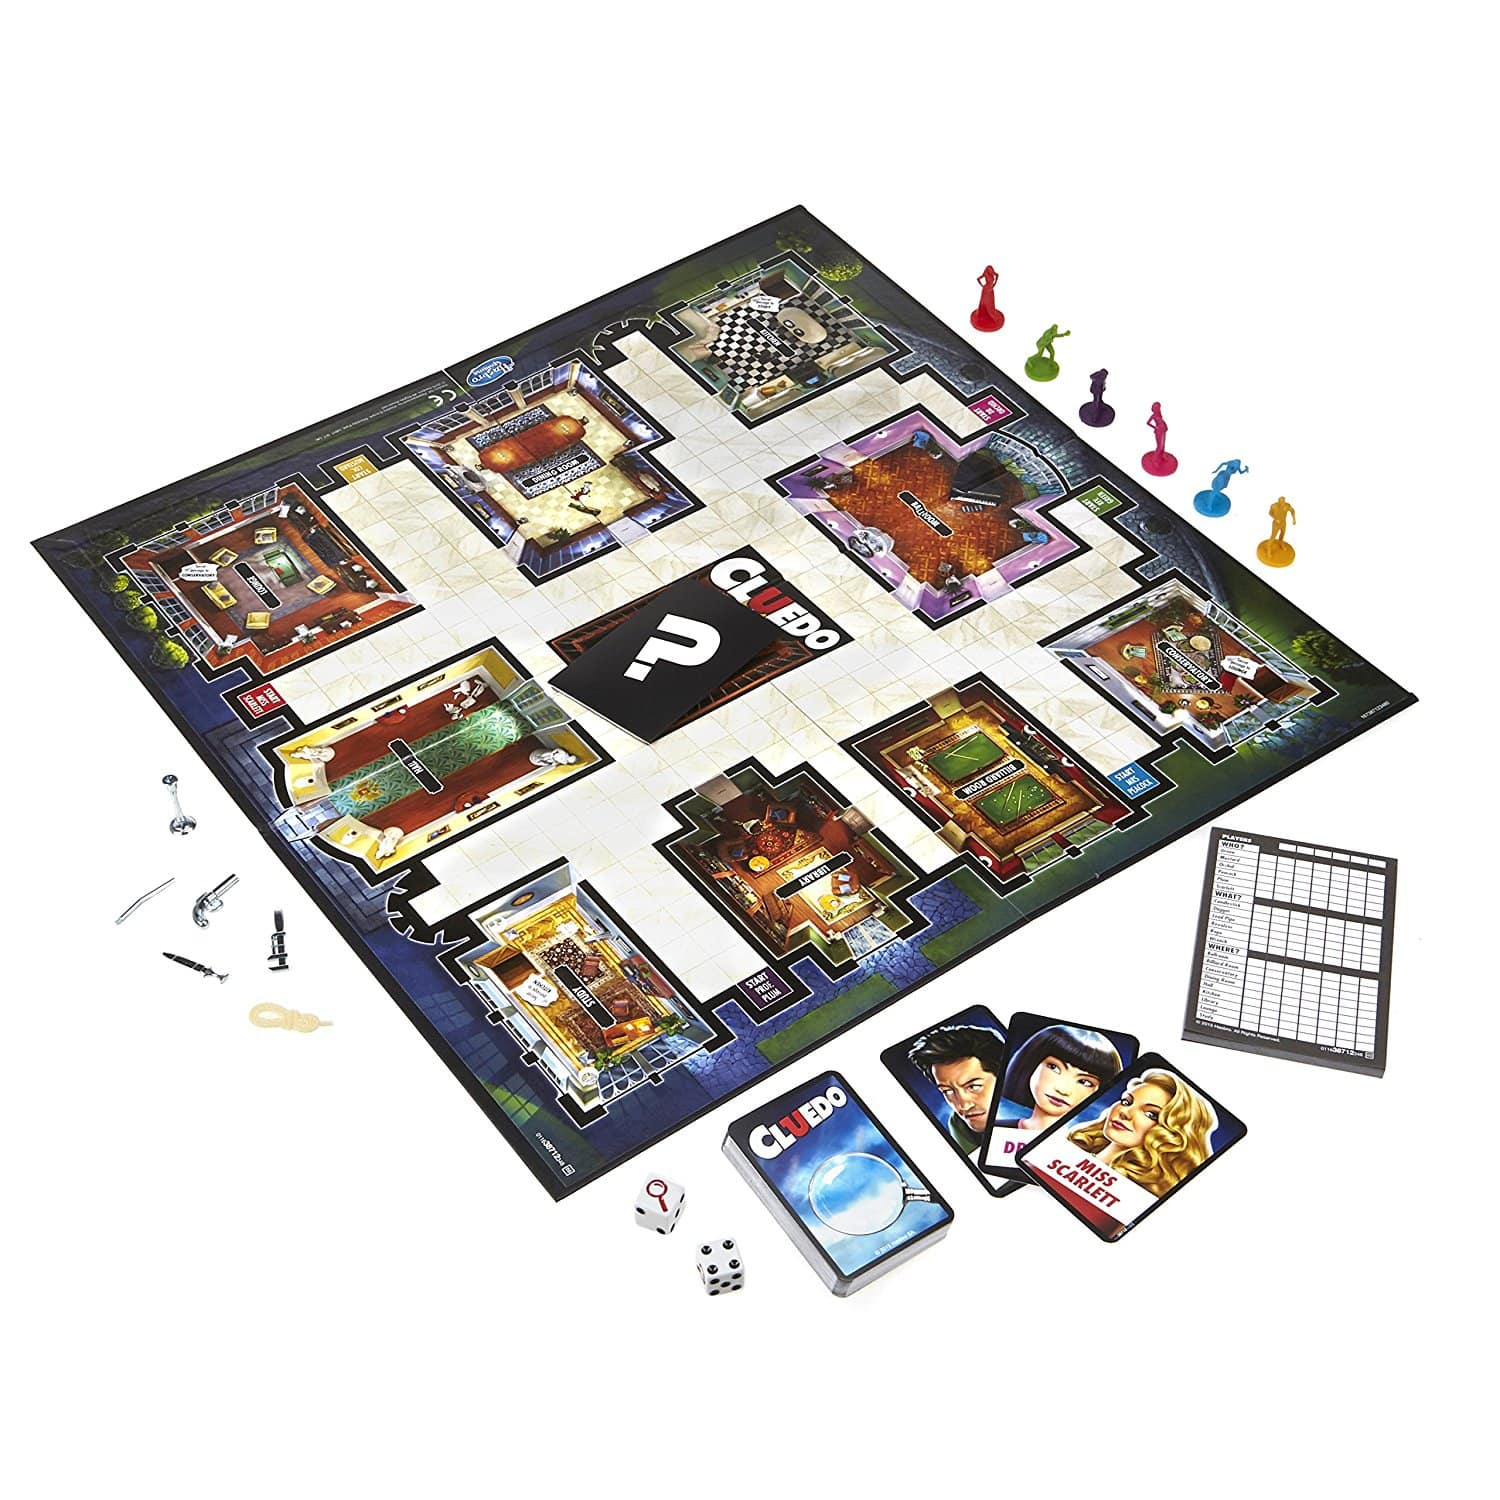
\includegraphics[scale=0.15]{cluedo-fisico}
  \caption{Imagen que muestra los elementos del juego de mesa Cluedo.\protect\footnotemark}
  \label{figura-cluedo-fisico}
\end{figure}

\footnotetext{\url{https://www.amazon.es/Hasbro-Gaming-38712546-Games-Cluedo/dp/B01CELLR22/ref=sr_1_3?s=toys&ie=UTF8&qid=1532779025&sr=1-3&keywords=cluedo}, Hasbro}

\section{ARCore}
ARCore es un SDK de Google para dispositivos móviles que utilizan el sistema operativo Android. Este SDK contiene las funciones necesarias para construir aplicaciones de realidad aumentada en dispositivos móviles normales sin necesidad de sensores especiales.\\

ARCore permite hacer un reconocimiento inteligente del mundo real que le rodea, puede detectar superficies e imagenes, y esto último es o que nos interesa, ya que esta detecciíon de imagenes nos permitirá aumentar un juego de mesa a partir del tablero.\\

La utilización de ARCore para desarrollar una versión aumentada del Cluedo nos permitirá a partir del tablero añadir elementos virtuales, y mediante el manejo de estos elementos virtuales o otros elementos fisicos como cartas que se introducen en el campo de visión de la cámara, se podrá interactuar con el juego obteniendo una experiencia realista a la vez que muy expectacular gracias a los elementos virtuales que se situan en el mundo real.

\section{Propuesta inicial del juego}
El juego consistirá en un tablero que contendrá habitaciones, sobre las que los jugadores se pueden desplazar.\\

Los jugadores tendrán que investigar los datos del crimen, al inicio del juego se establecerá aleatoriamente un asesino, un arma y una habitación, y para averiguar los datos de este crimen el usuario tendrá que realizar una acusación.\\

Para realizar una acusación el jugador tendrá que indicar un personaje, una arma y una habitación. En el caso de que acierte el jugador ha ganado, en caso de que falle el jugador se pasa al turno del siguiente.\\

Cada habitación tendrá una distancia con las otras, y el jugador lanzando los dados puede desplazarse a las habitaciones que este lanzamiento les permita. En caso de que obtenga un numero que no permite ir a ninguna habitación, se almacenará para la siguiente tirada de dados.\\

El jugador tiene que desplazarse entre las distintas habitaciones para obtener diferentes pistas en cada una de ellas, y las pistas serán diferentes para los distintos jugadores. Las pistas se mostrarán únicamente cuando el jugador llega a una habitación por primera vez.\\

Se podrá anotar información sobre los personajes/armas/habitaciones sospechosos, de forma que el jugador podrá marcar con una X si sabe seguro que ese personaje/arma/habitación, ayudando así a descubrir los datos del asesinato.

\subsection{Narrativa}
En la mansión de un aristocrata se celebra una fiesta, el anfitrión ha invitado a sus seis mejores amigos. Durante la velada uno de los amigos del anfitrión le asesina, en una habitación y con un arma específicos, los amigos encuentran el cadaver del anfitrión en el sótano y llaman a detectives para que investiguen el asesinato, de forma que ninguno de los amigos puede salir de la mansión hasta que se haya descubierto quien es el asesino.\\

El juego comienza cuando los detectives llegan a la mansión, estos detectives se tendrán que encargar de desplazarse por las diferentes habitaciones de la casa investigando hasta averiguar quien fue el asesino, con que arma cometio dicho asesinato y en que habitación.

\subsection{Realidad aumentada}
Este juego ofrece muchas posibilidades en la forma en la que implementarlo utilizando realidad aumentada, estas son las ideas iniciales sobre cómo implementar el juego con realidad aumentada:

\begin{itemize}
  \item Detectar el tablero de juego, y a partir de esta imagen mostrar los elementos, que incluyen personajes/habitaciones/armas 3D, en las habitaciones que le correspondan.
  \item Mostrar cartas en 3D alrededor del tablero de juego, que muestren las pistas mostradas al jugador actual, de forma que si una carta aparece es una pista indicando que el personaje/arma/habitación no ha cometido el asesinato.
  \item Mostrar diferente información a los difetentes jugadores, de forma que cuando se pase de turno, por ejemplo, las pistas sean diferentes para los diferentes jugadores, así tienen información diferente en función de como exploren las habitaciones cada uno.
  \item Mostrar los botones de funcionalidad, por ejemplo, el de pasar de turno o lanzar los dados como cubos 3D, que al tocarlos realizan dicha acción.
  \item Realizar las acusaciones con elementos físicos, es decir, que utilizando cartas reales de personajes/armas/habitaciones se pueda realizar una acusación, de forma que escaneando las 3 a la vez en la escena se realiza la acusación, permitiendo así un mejor balance entre la parte virtual del juego y la parte real.
\end{itemize}
